\documentclass{beamer}
\usepackage{hyperref}
\usepackage{url}
\usepackage{multimedia}
%\setbeamercovered{transparent}
%\beamertemplateshadingbackground{blue!5}{yellow!10}
\usepackage{beamerthemesplit}
\usepackage{algorithmic}
\usepackage{epsfig,amsfonts,amsmath,amstext,amssymb,latexsym}
\begin{document}
\title[Healthcare Intervention in Local Hospitals]
{Healthcare Intervention in Local Hospitals
}
\author[\insertframenumber/\inserttotalframenumber
\hspace{1in} Saket Choudhary]
{Saket Choudhary \\
}
%\today{} 
\begin{frame}
   \titlepage
\vspace{-1cm}

\end{frame}

\begin{frame}
\frametitle{Motivation \& Goal}
    \begin{itemize}
        \item The  field of healthcare is a ground to number of problems with a potential 'engineering solution'
        \item The problems are best understood by interacting with the clinicians at local hospitals 
        \item Visit local hospitals like TMH, Hinduja to find out what possible engineering solution can be delieverd 
    \end{itemize}
\end{frame}

\begin{frame}
\frametitle{Details}
    \begin{itemize}
        \item  Made two visits to Hinduja Hospital
        \item  Interacted with Dr. Devendra Desai , Gastroenterologist
        \item  Interacted with Dr. R B Deshpande,  Histopathologist
    \end{itemize}
\end{frame}


\begin{frame}[allowframebreaks]
\frametitle{Image analysis of digitised Tuberculosis smear samples : The Problem}
\begin{figure}[!h]
    \begin{center}
        \scalebox{0.75}{
			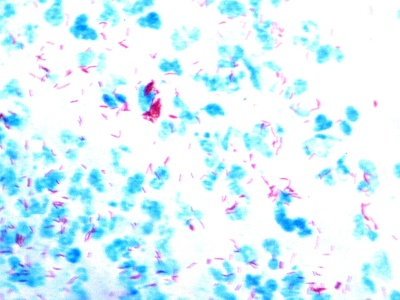
\includegraphics{afb1-small.JPG}}
    \end{center}
    		\caption{Digital Image of a TB Smear Slide}
\end{figure}
    \begin{itemize}
        \item  It is possible to digitise the TB smear  slides in the form of images
        
        
        \item  The images further can be analysed using a software that would mark out the positions of the bacteria 
        \item  The analysis differs from one clinican to the other because of the different perception of colours
        
        \item  This would help the clinicians to study the TB samples even remotely
        \item A digital image can be easily shared between doctors and the doctors can pass on their individual feedback after analysing the image through this image-analysis package
        

    \end{itemize}
\end{frame}

\begin{frame}
\frametitle{The Solution}
    \begin{itemize}
        \item  A cross platform GUI to analyse images
        \item  The software allows loading files , perform analysis on images and mark the regions of interest
        \item  The resulting image can be visualised  side by side  with the original to get an idea  of the potentials spots where bacterium could be present
        \item  Since the perception of 'pink' differs from  cliniclan to clinician to adjust the cutoff levels for image segmentation based on 'pink' color
    \end{itemize}
\end{frame}

\begin{frame}[allowframebreaks]
\begin{figure}[!h]
    \begin{center}
        \scalebox{0.32}{
			\includegraphics{first.png}}
    \end{center}
    		\caption{The File Chooser and the Threshold adjuster}
\end{figure}

\begin{figure}[!h]
    \begin{center}
        \scalebox{0.32}{
			\includegraphics{second.png}}
    \end{center}
    		\caption{Loading Image by Selecting the File}
\end{figure}


\begin{figure}[!h]
    \begin{center}
        \scalebox{0.32}{
			\includegraphics{third.png}}
    \end{center}
    		\caption{Detecting Edges }
\end{figure}


\begin{figure}[!h]
    \begin{center}
        \scalebox{0.32}{
			\includegraphics{fourth.png}}
    \end{center}
    		\caption{The Resulting Image }
\end{figure}

\end{frame}

\begin{frame}
\frametitle{Possible Improvements}
    \begin{itemize}
	\item Zoom Option
	\item Neater GUI
	\item Enhance the contrast for the result image
	\item Clinician Feedback and Machine Learning
	\item  Direct image sharing by email/internet
	\item Subpart of the the automation machinery
	
	

    \end{itemize}
        
\end{frame}




\begin{frame}
\center
We zeroed upon solving the Image Analysis Problem as it seemed more feasible  from an implmentation point of view . 
As part of my trip  to Hinduja Hosptials,  I also made a list of other problems that require an engineering solution in the following slides
\end{frame}



\begin{frame}
\frametitle{Ideas : An  Indian Endoscope}
    \begin{itemize}
        \item  Endoscopy involves examining the hollow organs of the body through an ‘endoscope’
        \item  Endoscopes used today in India are imported from foreign countries
        \item  The challenge is to come with low-cost version of the endoscope and its accessories
    \end{itemize}
\end{frame}





\begin{frame}
\frametitle{Ideas : Telemedicine}
    \begin{itemize}
        \item  There is a tremendous amount of scope that can be used to improve the doctor-patient interaction through telemedicine
        \item  A doctor sitting at a hospital can provide consultation to the patient from a remote health centre through an audio-video call
        \item  A software that would have features like video/audio conferencing, sharing reports/X-ray images in realtime and realtime feedback system 
    \end{itemize}
\end{frame}



\begin{frame}
\frametitle{Ideas : Automation of Tuberculosis detection from smear samples}
    \begin{itemize}
        \item  The current setup of detecting TB involves the clinician loading the slides on to the microscope , then manually move the slides under the lens till a 
pink dot’(if exists) is visible
        \item   Being a manual process it may take several minutes before the clinician strikes at the location where bacterium might be present
        \item  There is a scope for automation here where a robot would pick up a slide from a stack of slides , one by one, adjust it under the lens till a ‘pink spot’ is visible and mark this position 
        \item The clinican can then just look at these dots and decide if the bacterium is present
        \item . This will considerably reduced the time spent per sample and thus would lead to a speedy diagnosis
    \end{itemize}
\end{frame}




\begin{frame}
\frametitle{Image analysis of digitised Tuberculosis smear samples}
    \begin{itemize}
	\item The bacilli are differently coloured then the rest of the sample
	\item Perform color based image segmentation to separrate the bacilli from the rest of the sample
	\item The input for threshold values comes from the user
	\item Directory based listing of images
	\item Side by Side images for comparison
	\item Uses open source python-libraries : wx, opencv
	\item Implementations of similar software uses either MATLAB based solutions or machine learning approach
	

    \end{itemize}
\end{frame}




\begin{frame}
\frametitle{Conclusions}
    \begin{itemize}
	\item An Open source  and cross platform solution
	\item Currently in its POC stage
	\item Needs many iterations for development
	\item Better Algorithms possible 
	
	

    \end{itemize}
        
\end{frame}




\end{document}
